% Auto-generated graph inspection block.
\subsection{Graph Inspection}
The generated syscall graphs remain in a small-to-medium regime while staying fairly dense: ADFA-LD contains 5951 graphs with 19.9 nodes and 57.3 edges on average (directed density 0.245); LID-DS (Bruteforce\_CWE-307) contains 907 graphs with 29.5 nodes and 240.5 edges on average (directed density 0.283); LID-DS (CVE-2014-0160) contains 878 graphs with 29.8 nodes and 113.8 edges on average (directed density 0.132). This profile makes local message-passing models appropriate because each node interacts with a limited but informative neighborhood, so a few propagation steps can aggregate most of the useful local transition context without requiring very deep architectures. We therefore compare a plain GCN baseline, GraphSAGE for more robust neighborhood aggregation, GAT to test whether attention over heterogeneous syscall transitions improves discrimination, and our WGCN+ variant that combines weighted GCN propagation, learned syscall embeddings, structural node features, layer normalization, and hybrid graph pooling.

\begin{table}[H]
\centering
\resizebox{\linewidth}{!}{%
\begin{tabular}{lrrrrrr}
\hline
Dataset & Graphs & Attack \% & Mean $|V|$ & Mean $|E|$ & Mean density & Mean seq. len. \\
\hline
ADFA-LD & 5951 & 12.54 & 19.94 & 57.29 & 0.24 & 461.70 \\
LID-DS (Bruteforce\_CWE-307) & 907 & 15.33 & 29.47 & 240.53 & 0.28 & 8136.46 \\
LID-DS (CVE-2014-0160) & 878 & 13.67 & 29.78 & 113.81 & 0.13 & 1640.26 \\
\hline
\end{tabular}
}
\caption{Graph-level inspection of the datasets used by the training pipeline, computed on the same trace pools as the reported experiments.}
\label{tab:graph-inspection}
\end{table}

\begin{figure}[H]
\centering
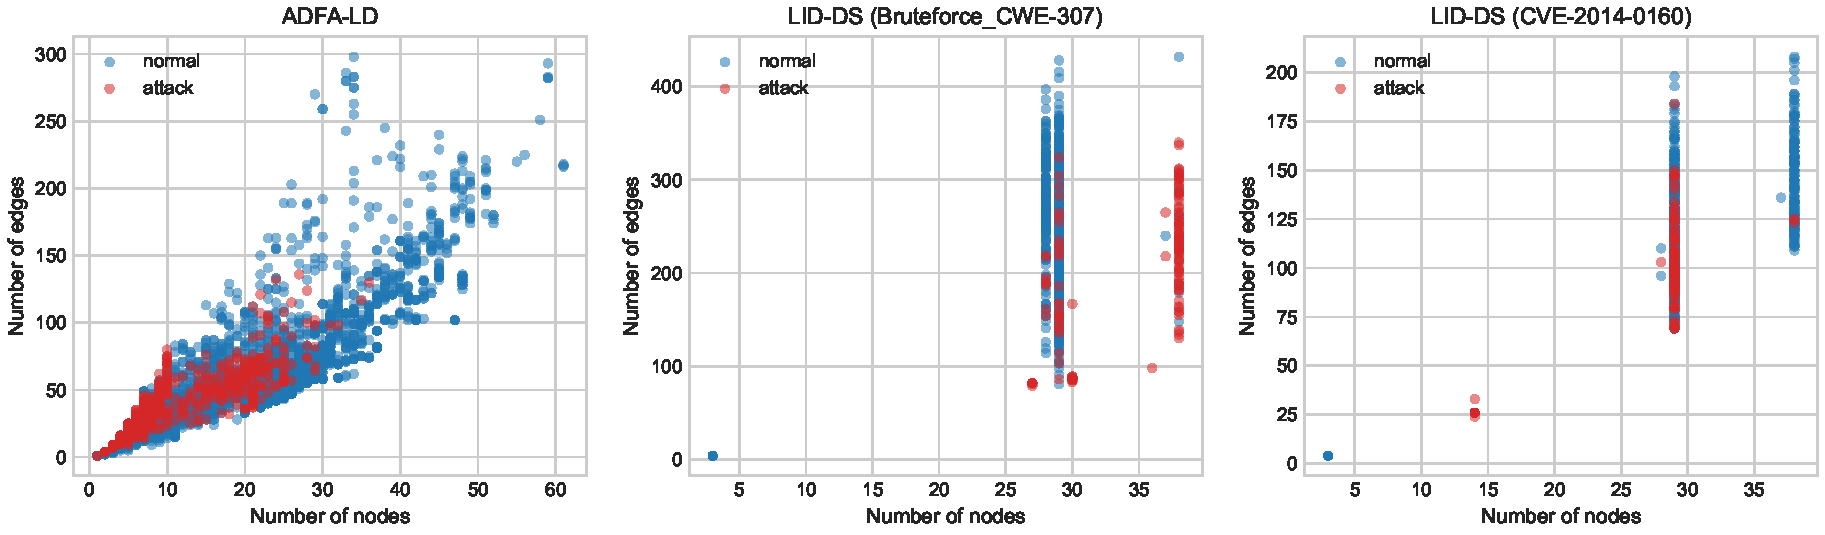
\includegraphics[width=0.72\linewidth]{figures/graph_nodes_edges_scatter.pdf}
\caption{Number of nodes versus number of edges for the generated syscall graphs, colored by class.}
\label{fig:graph-inspection}
\end{figure}
